\documentclass{beamer}
\usepackage{graphicx}
\usepackage{listings}
\usepackage{amsfonts}
\usepackage{amsmath}
\usepackage{multicol}
\usepackage[pdf]{graphviz}
\usepackage[skins,breakable,listings]{tcolorbox}

\lstset{basicstyle=\ttfamily,breaklines=true}
\usepackage{upquote}
%\def\backtick{\char18}
\lstdefinestyle{backtickstyle}{literate={`}{\char}1, escapechar=@}

\usepackage{fontspec}

\makeatletter
\def\verbatim@nolig@list{}
\makeatother

\setmonofont{JetBrains Mono}[Contextuals=Alternate]

\usepackage{ocr}
\usepackage[T1]{fontenc}

%\usepackage{cmap} % Copy-pastable unicode characters
\usepackage{epigraph}
\usepackage{accsupp}
\usepackage{bussproofs}
\newcommand{\noncopyable}[1]{%
\BeginAccSupp{method=escape,ActualText={}}%
#1%
\EndAccSupp{}%
}

\lstdefinelanguage{kotlin}{
comment=[l]{//},
commentstyle={\color{gray}\ttfamily},
emph={delegate, filter, firstOrNull, forEach, it, lazy, mapNotNull, println, repeat, assert, with, head, tail, len, return@},
numberstyle=\noncopyable,
emphstyle={\color{olive}},
identifierstyle=\color{black},
keywords={abstract, actual, as, as?, break, by, class, companion, continue, data, do, dynamic, else, enum, expect, false, final, for, fun, get, if, import, in, infix, interface, internal, is, null, object, open, operator, override, package, private, public, return, sealed, set, super, suspend, this, throw, true, try, catch, typealias, val, var, vararg, when, where, while, tailrec, reified, Repeat},
keywordstyle={\color{blue}\bfseries},
morecomment=[s]{/*}{*/},
morestring=[b]",
morestring=[s]{"""*}{*"""},
ndkeywords={@Deprecated, @JvmField, @JvmName, @JvmOverloads, @JvmStatic, @JvmSynthetic, Array, Byte, Double, Float, Boolean, Int, Integer, Iterable, Long, Runnable, Short, String, Pair},
ndkeywordstyle={\color{purple}\bfseries},
sensitive=true,
stringstyle={\color{green}\ttfamily},
literate={`}{{\char0}}1
}

\newtcblisting{kotlinlisting}[1][]{%
listing options={
language=kotlin,
basicstyle=\scriptsize\ttfamily,
%numberstyle=\footnotesize\noncopyable,
showstringspaces=false,
tabsize=2,
breaklines=true,
%numbers=right,
inputencoding=utf8,
escapeinside={(*@}{@*)},
#1
},
underlay unbroken and first={%
\path[draw=none] (interior.north west) rectangle node[white]{\includegraphics[width=4mm]{../figures/kotlin_file.png}} ([xshift=-10mm,yshift=-12mm]interior.north west);
}
}

\tcbset{
enhanced jigsaw,
listing only,
%boxsep=-1pt,
%top=-1pt,
%bottom=-0.5pt,
center,
width=0.92\textwidth,
%right=-0.5pt,
overlay first={
\node[black!50] (S) at (frame.south) {\Large\ding{34}};
\draw[dashed,black!50] (frame.south west) -- (S) -- (frame.south east);
},
overlay middle={
\node[black!50] (S) at (frame.south) {\Large\ding{34}};
\draw[dashed,black!50] (frame.south west) -- (S) -- (frame.south east);
\node[black!50] (S) at (frame.north) {\Large\ding{34}};
\draw[dashed,black!50] (frame.north west) -- (S) -- (frame.north east);
},
overlay last={
\node[black!50] (S) at (frame.north) {\Large\ding{34}};
\draw[dashed,black!50] (frame.north west) -- (S) -- (frame.north east);
},
before={\par\vspace{10pt}},
after={\par\vspace{10pt}\noindent}
}

\newcommand*{\inlineimg}[1]{%
\raisebox{-.3\baselineskip}{%
\includegraphics[
height=\baselineskip,
width=\baselineskip,
keepaspectratio,
]{#1}%
}%
}

\definecolor{slightgray}{rgb}{0.90, 0.90, 0.90}

\usepackage{soul}
\usepackage{hyperref}
\makeatletter
\def\SOUL@hlpreamble{%
\setul{}{3.0ex}%
\let\SOUL@stcolor\SOUL@hlcolor%
\SOUL@stpreamble%
}
\makeatother

\newcommand{\inline}[1]{%
\begingroup%
\sethlcolor{slightgray}%
\hl{\ttfamily\footnotesize #1}%
\endgroup
}

\newcommand{\tinline}[1]{%
\begingroup%
\sethlcolor{slightgray}%
\hl{\ttfamily\tiny #1}%
\endgroup
}

\mode<presentation> { \usetheme{Madrid} }

\title{Pattern Recognition in Procedural Knowledge}
\subtitle{Comprehensive Exam}

\author{Breandan Considine}

\institute[McGill]{
McGill University \\
\medskip
\textit{breandan.considine@mcgill.ca}
}
\date{\today}


\begin{document}
  \begin{frame}
    \titlepage
  \end{frame}

  \begin{frame}
    \frametitle{Knowledge is lost in translation}
    \begin{itemize}
      \item First an end user describes a problem using natural language
      \item Next an expert translates the problem into a formal language
      \item Then an engineer implements the spec in a programming language
      \item Code is \textit{not} the model, just one implementation of the model
      \item And the model itself is just an approximation of the real world
      \item System identification is hard, most abstractions are leaky
    \end{itemize}
    \begin{figure}[H]
      \centering
      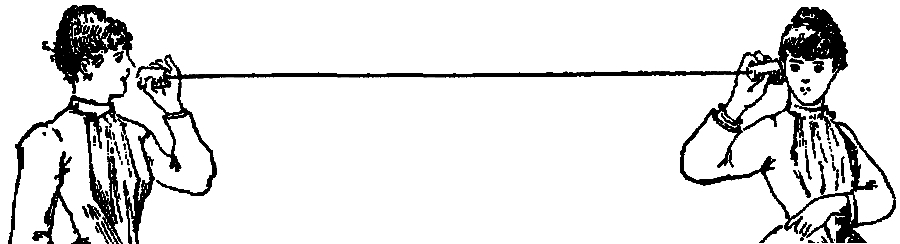
\includegraphics[width=0.8\textwidth]{../clipart/tincan.jpg}
    \end{figure}
  \end{frame}

  \begin{frame}
    \frametitle{Knowledge is difficult to grasp}
    \begin{itemize}
      \item The human neocortex has a finite capacity working memory
      \item Many codebases are enormous bodies of collective knowledge
      \item Cannot be grasped entirely by a single knowledge worker
      \item Programs do not live on a computer, programs are abstract concepts
      \item Code is simply one \textit{artifact} or byproduct of computer programming
      \item Seek to understand the creative process, not the byproduct
    \end{itemize}
    \begin{figure}[H]
      \centering
      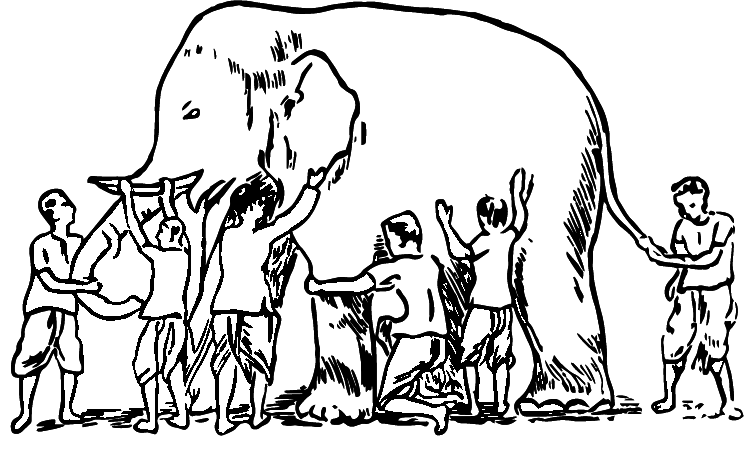
\includegraphics[width=0.5\textwidth]{../clipart/elephant.png}
    \end{figure}
  \end{frame}

  \begin{frame}
    \frametitle{Knowledge does not compose}
    \begin{itemize}
      \item Complex systems require participation from many stakeholders
      \item In order to scale up participation, we need programs to compose
      \item Impossible to build complex systems by cobbling together spare parts
      \item Need better ways to facilitate collaborative knowledge engineering
    \end{itemize}
    \begin{figure}[H]
      \centering
      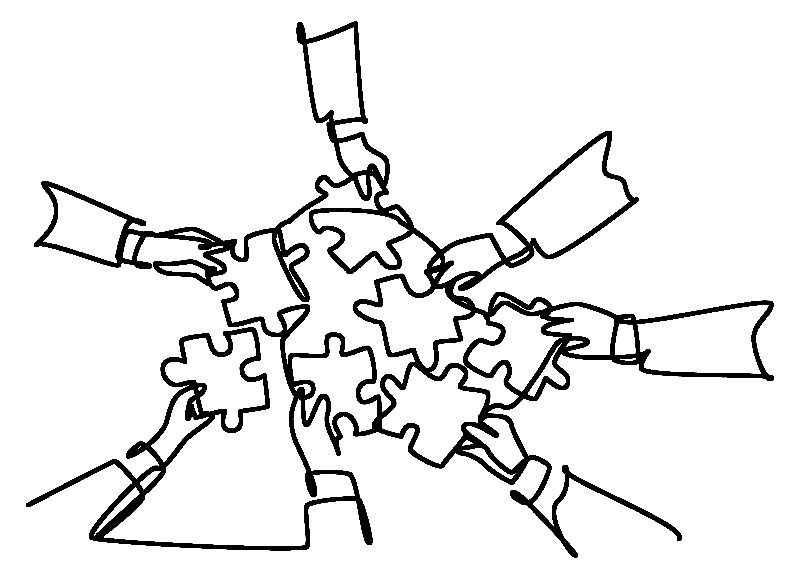
\includegraphics[width=0.5\textwidth]{../clipart/compositionality.jpeg}
    \end{figure}
  \end{frame}

  \begin{frame}
    \frametitle{Reason is a ladder to higher knowledge}
    \begin{itemize}
      \item To facilitate human understanding, we must have better tools
      \item Tools should complement, not supplant human reasoning abilities
      \item Reasoning is a tool to access higher forms of knowledge
      \item Seek to augment human intelligence by automated reasoning
    \end{itemize}
    \begin{figure}[H]
      \centering
      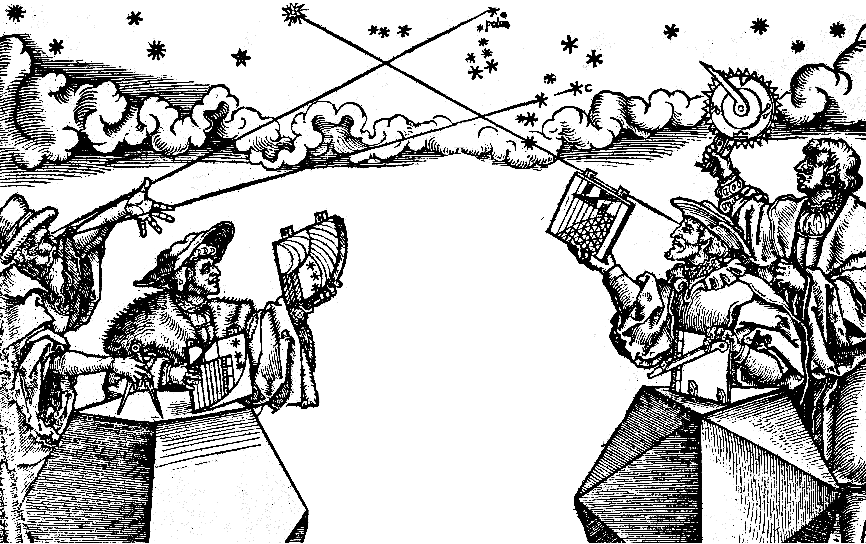
\includegraphics[width=0.5\textwidth]{../clipart/astronomers.png}
    \end{figure}
  \end{frame}

  \begin{frame}
    \frametitle{Learning and reasoning from first principles}
    \begin{itemize}
%      \item Learning to program by reading trillions of lines of code is like
%      \\Learning to drive by reading highway transportation law
      \item Learning to program by imitating big code is a hopeless task!
      \item Such a system will only generate more code, increase technical debt
      \item Source code alone is fragile, contains too many brittle assumptions
      \item Where does source code come from? Need to retrace its provenance
      \item Software more than just source code, many supporting artifacts
      \item Software engineering starts with pen and paper\ldots
    \end{itemize}
    \begin{figure}[H]
      \centering

      \begin{prooftree}
        \bottomAlignProof
        \AxiomC{}
        \UnaryInfC{$a \sim a$}
        \noLine
        \UnaryInfC{}
        \noLine
        \UnaryInfC{\textit{Reflexivity}}
        \DisplayProof
        \hskip 1.5em
        \bottomAlignProof
        \AxiomC{$a \sim b$}
        \UnaryInfC{$b \sim a$}
        \noLine
        \UnaryInfC{}
        \noLine
        \UnaryInfC{\textit{Symmetry}}
        \DisplayProof
        \hskip 1.5em
        \bottomAlignProof
        \AxiomC{$a \sim b$}
        \AxiomC{$b \sim c$}
        \BinaryInfC{$a \sim c$}
        \noLine
        \UnaryInfC{}
        \noLine
        \UnaryInfC{\textit{Transitivity}}
        \DisplayProof
        \hskip 1.5em
        \bottomAlignProof
        \AxiomC{$a \sim b$}
        \UnaryInfC{$f(a) \sim f(b)$}
        \noLine
        \UnaryInfC{}
        \noLine
        \UnaryInfC{\textit{Congruence}}
      \end{prooftree}

    \end{figure}
  \end{frame}

  \begin{frame}
    \frametitle{Induction, Deduction, Abduction, Transduction, et al.}
    \begin{itemize}
      \item \textbf{*duction}: From Latin ductio, ductionem, meaning to lead away
      \item \textbf{Conduction}: Transfer energy from one location to another
      \item \textbf{Induction}: Infer general rules from specific observations
      \item \textbf{Deduction}: Infer specific predictions from general rules
      \item \textbf{Abduction}: Infer higher order rules (theory) from specific facts
      \item \textbf{Transduction}: Infer specific predictions from specific observations
      \item \textbf{Production}: Infer a more complex expression from a simpler one
      \item \textbf{Reduction}: Infer a more simple expression from a more complex one
    \end{itemize}
    % http://web.cecs.pdx.edu/~harry/discrete/slides/Section3.1.pdf
    \begin{figure}[H]
      \centering
      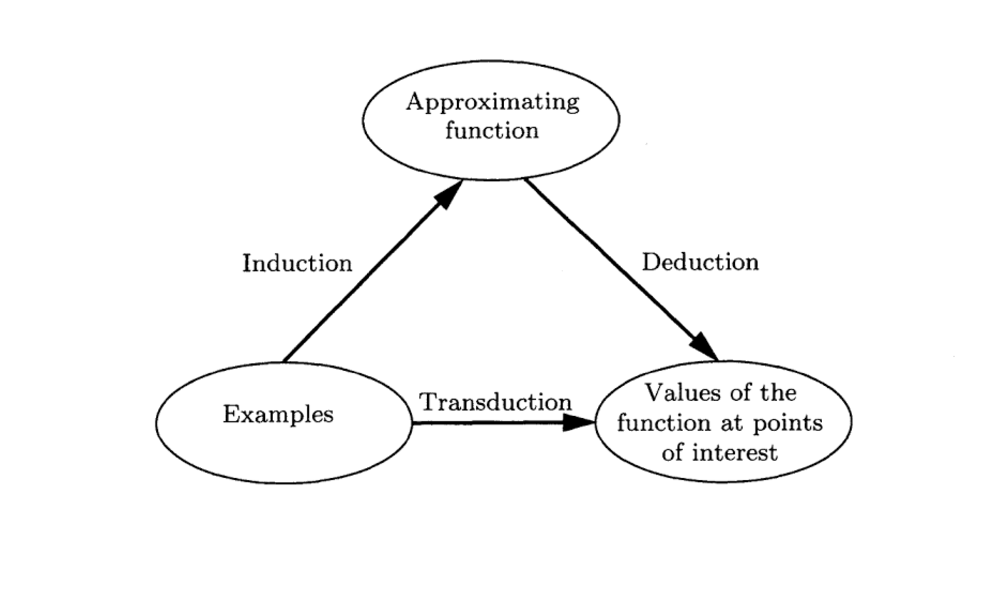
\includegraphics[width=0.3\textwidth]{../clipart/induction_deduction_transduction.png}
      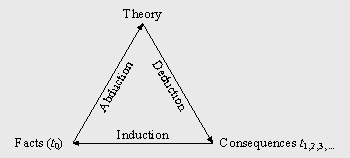
\includegraphics[width=0.3\textwidth]{../clipart/induction_deduction_abduction.png}
    \end{figure}
  \end{frame}

  \begin{frame}[fragile]
    \frametitle{Logical Induction}
    \begin{itemize}
      \item Inductive data types: $\texttt{type Nat = Zero | Succ Nat}$
      \item Inductive/recursive definitions: basis, induction, closure
      \item Sum-Product networks:
      \begin{lstlisting}
      type SPN = SimpleDistribution
               | + (SPN a) (SPN a)
               | * (SPN a) (SPN a)
      \end{lstlisting}
      \item Inductively defined graphs:
      \begin{lstlisting}
      type Graph = Empty | Vertex
                 | + (Graph a) (Graph a)
                 | * (Graph a) (Graph a)
      \end{lstlisting}
      \item Coinduction / corecursion
    \end{itemize}
    % https://shmorhay.wordpress.com/2017/10/20/machine-learning-abduction-and-transduction/
    % http://www.jfsowa.com/talks/iccs03.htm
  \end{frame}

  \begin{frame}
    \frametitle{Induction in Machine Learning}
    \begin{itemize}
      \item How should machine learners fill in the gaps between observations?
      \item Inductive biases allow a learning algorithm to prioritize one solution or interpretation over another, irrespective of the observed data, e.g.:
      \begin{itemize}
        \item Risk minimization (Vapnik, Chervonenkis, Arjovsky, et al.)
        \item Minimum description length (Solomonoff, Kolmogorov, Chaitin)
        \item Maximum entropy (Shannon, Jaynes et al.)
        \item Nearest neighbors (Fix, Hodges, Cover et al.)
%        \item Relational inductive biases (Battaglia et al.)
        % https://blog.acolyer.org/2018/09/19/relational-inductive-biases-deep-learning-and-graph-networks/
        \end{itemize}
    \end{itemize}
    \begin{figure}[H]
      \centering
      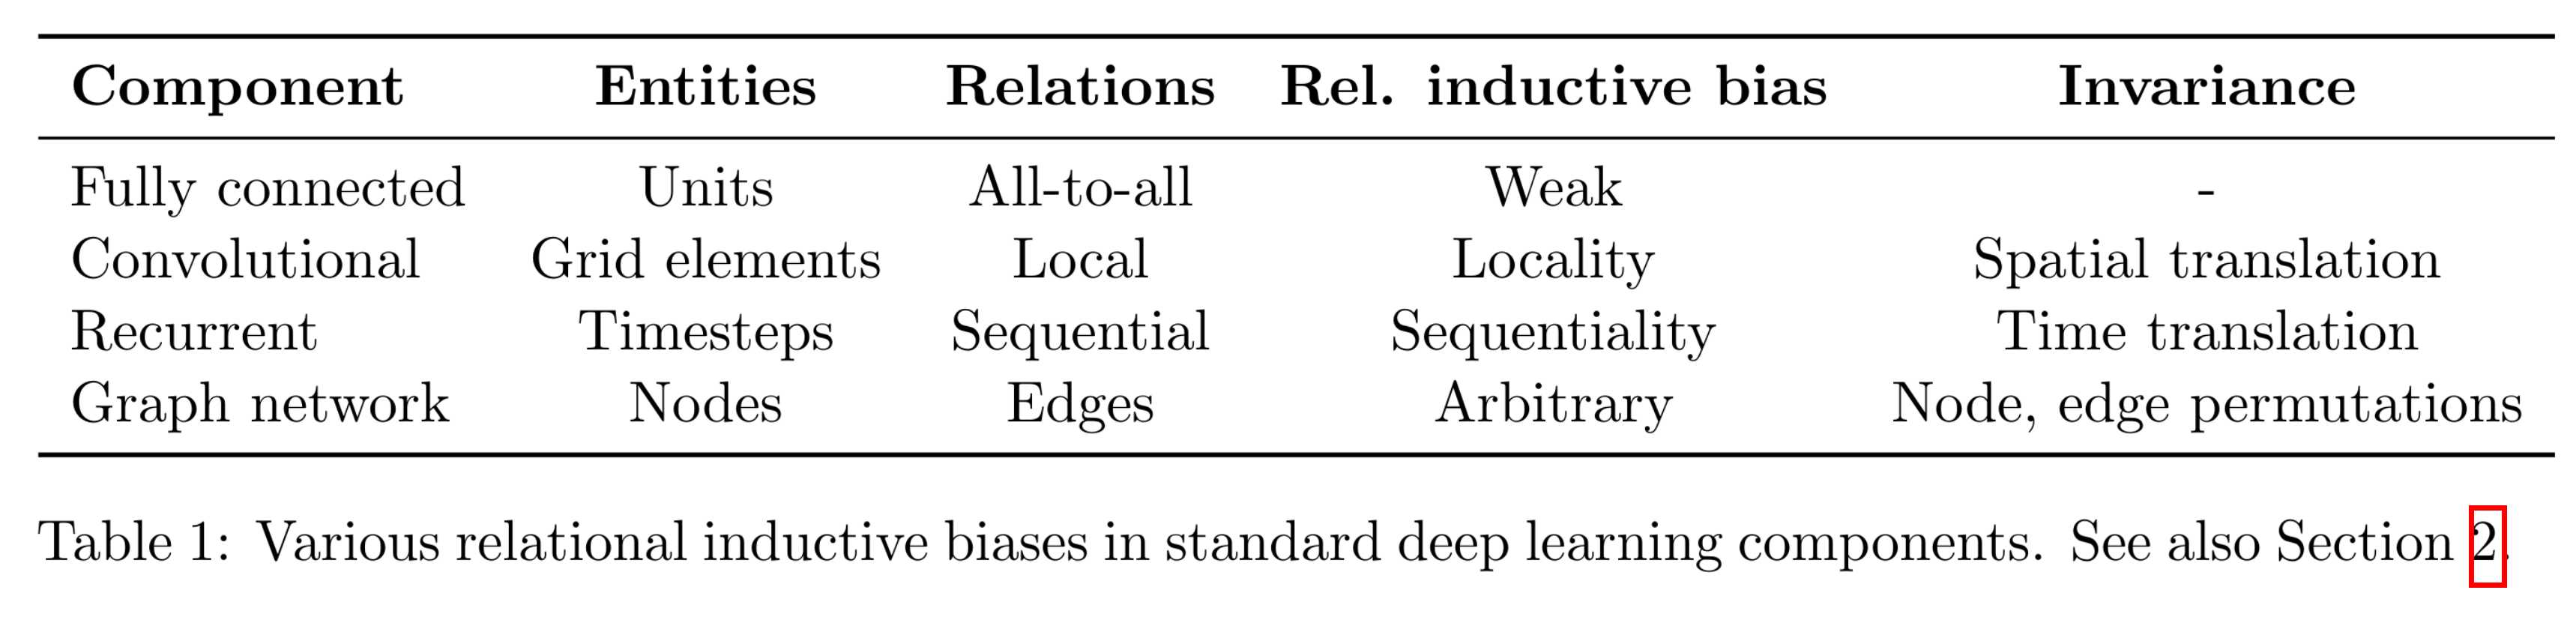
\includegraphics[width=0.9\textwidth]{../clipart/relational_inductive_biases.jpg}
      \caption{From \href{https://arxiv.org/pdf/1806.01261.pdf}{Battaglia et al. (2018), ``Relational inductive biases''}}
    \end{figure}
  \end{frame}

  \begin{frame}
    \frametitle{What do these two formalisms share in common?}
    \begin{itemize}
      \item Propagate information through some kind of graph
      \item Circuits propagate electricity through a copper graph
%      \item BNNs propagate electrochemical impulses through a cellular graph
      \item Proofs propagate propositions through a logical graph
      \item Neural networks propagate error through a computation graph
      \item Bayes networks propagate uncertainty through a probabilistic graph
%      \item Citation networks propagate ideas through a citation graph
%      \item $\lambda$-calculus propagates $\lambda$ terms through a reduction graph
    \end{itemize}
    \begin{figure}[H]
      \centering
      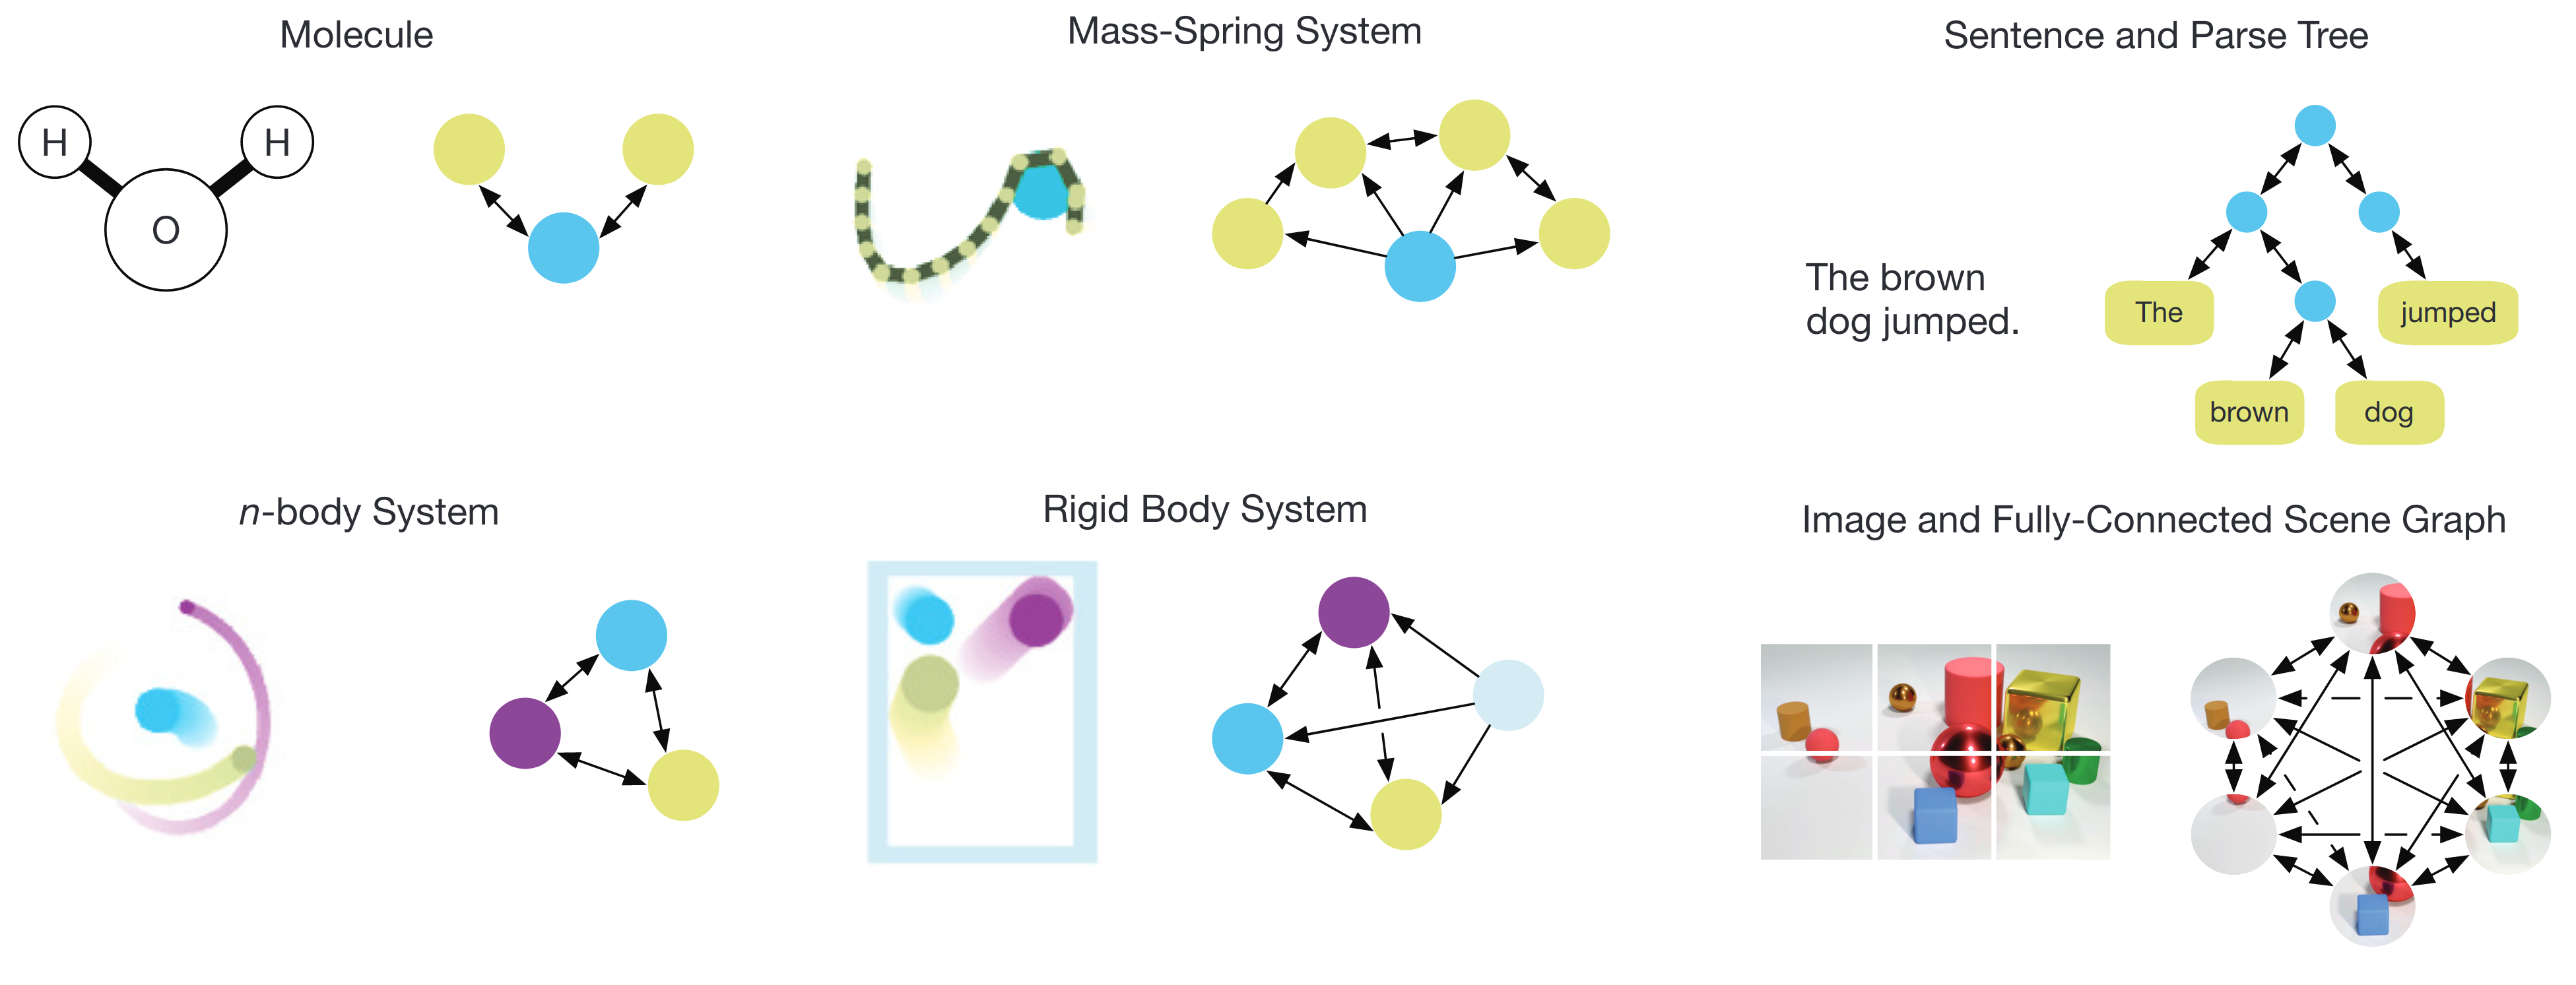
\includegraphics[width=0.8\textwidth]{../clipart/relational_biases.png}
      \caption{From \href{https://arxiv.org/pdf/1806.01261.pdf}{Battaglia et al. (2018), ``Relational inductive biases''}}
    \end{figure}

  \end{frame}

  \begin{frame}
    \frametitle{Static versus dynamic graphs}
    \begin{itemize}
      \item Sometimes the graph is static (matrix multiplication)
      \item Just propagate simple values through it (e.g. $\mathcal{T} \in {\mathbb{R, B, Z, C}}$)
      \item Sometimes the graph is dynamic (tensor contraction)
      \item Can propagate more complex objects (e.g. $\mathcal{T}^2, \mathcal{T}^3, \mathcal{T}^k$)
      \item Hyper-graph/edge replacement grammars (HRGs, FGGs, GGs et al.)
    \end{itemize}
  \end{frame}

  \begin{frame}
    \frametitle{The algebra of graph replacement}
    \begin{itemize}
      \item Semiring algebras (Gondran and Minoux)
      \item Graph grammars (Ariola, Plump et al.)
      \item Basically generalizes linear algebra to other structures
    \end{itemize}
  \end{frame}

  \begin{frame}
    \frametitle{Valid and invalid procedures}
    \begin{itemize}
      \item Not all procedural text is source code
      \item Not all source code is syntactically valid / well-formed
      \item Not all well-formed programs are semantically valid
      \item Not all semantically valid programs are error-free
      \item Not all error-free programs terminate
      \item Not all terminating programs yield the correct answer
      \item Not only "not all", but uncountably many counterexamples
      \item Unconstrained sampling is doomed to fail
    \end{itemize}
  \end{frame}

  \begin{frame}
    \frametitle{Necessary assumptions}
    \setlength{\epigraphwidth}{0.5\textwidth}
    \epigraph{The expressive power of a programming language arises from its strictures and not from its affordances.}{Robert Harper}
    \begin{itemize}
      \item Bounded depth circuits
      \item Finite sample space
      \item All programs terminate
    \end{itemize}
  \end{frame}

  \begin{frame}
    \frametitle{The trouble with pattern recognition: Part I}
    \begin{itemize}
      \item Similar functions, dissimilar forms
      \item P1: Two functions may share the same meaning, but different forms
      \item E1: two programs may implement the exact same function, but share almost no syntax in common
      \item Q1: How do we recognize superficially dissimilar structures which share hidden meaning?
    \end{itemize}
  \end{frame}

  \begin{frame}
    \frametitle{The trouble with pattern recognition: Part II}
    \begin{itemize}
      \item Similar forms, dissimilar functions
      \item P2: Two objects may have a common form, but have vastly different meanings
      \item E2: two programs may differ by only a few tokens, but have drastically different meanings
      \item Q2: How do we disambiguate superficially similar structures?
    \end{itemize}
  \end{frame}

  \begin{frame}
    \frametitle{Relations among probability distributions}
    \begin{itemize}
      \item Knowledge is accumulated across generations of research
      \item Patterns have specific names, e.g. ``Gaussian'', ``Dirichlet''...
      \item Can we recover these relations from first principles?
    \end{itemize}
    \begin{figure}[H]
      \centering
      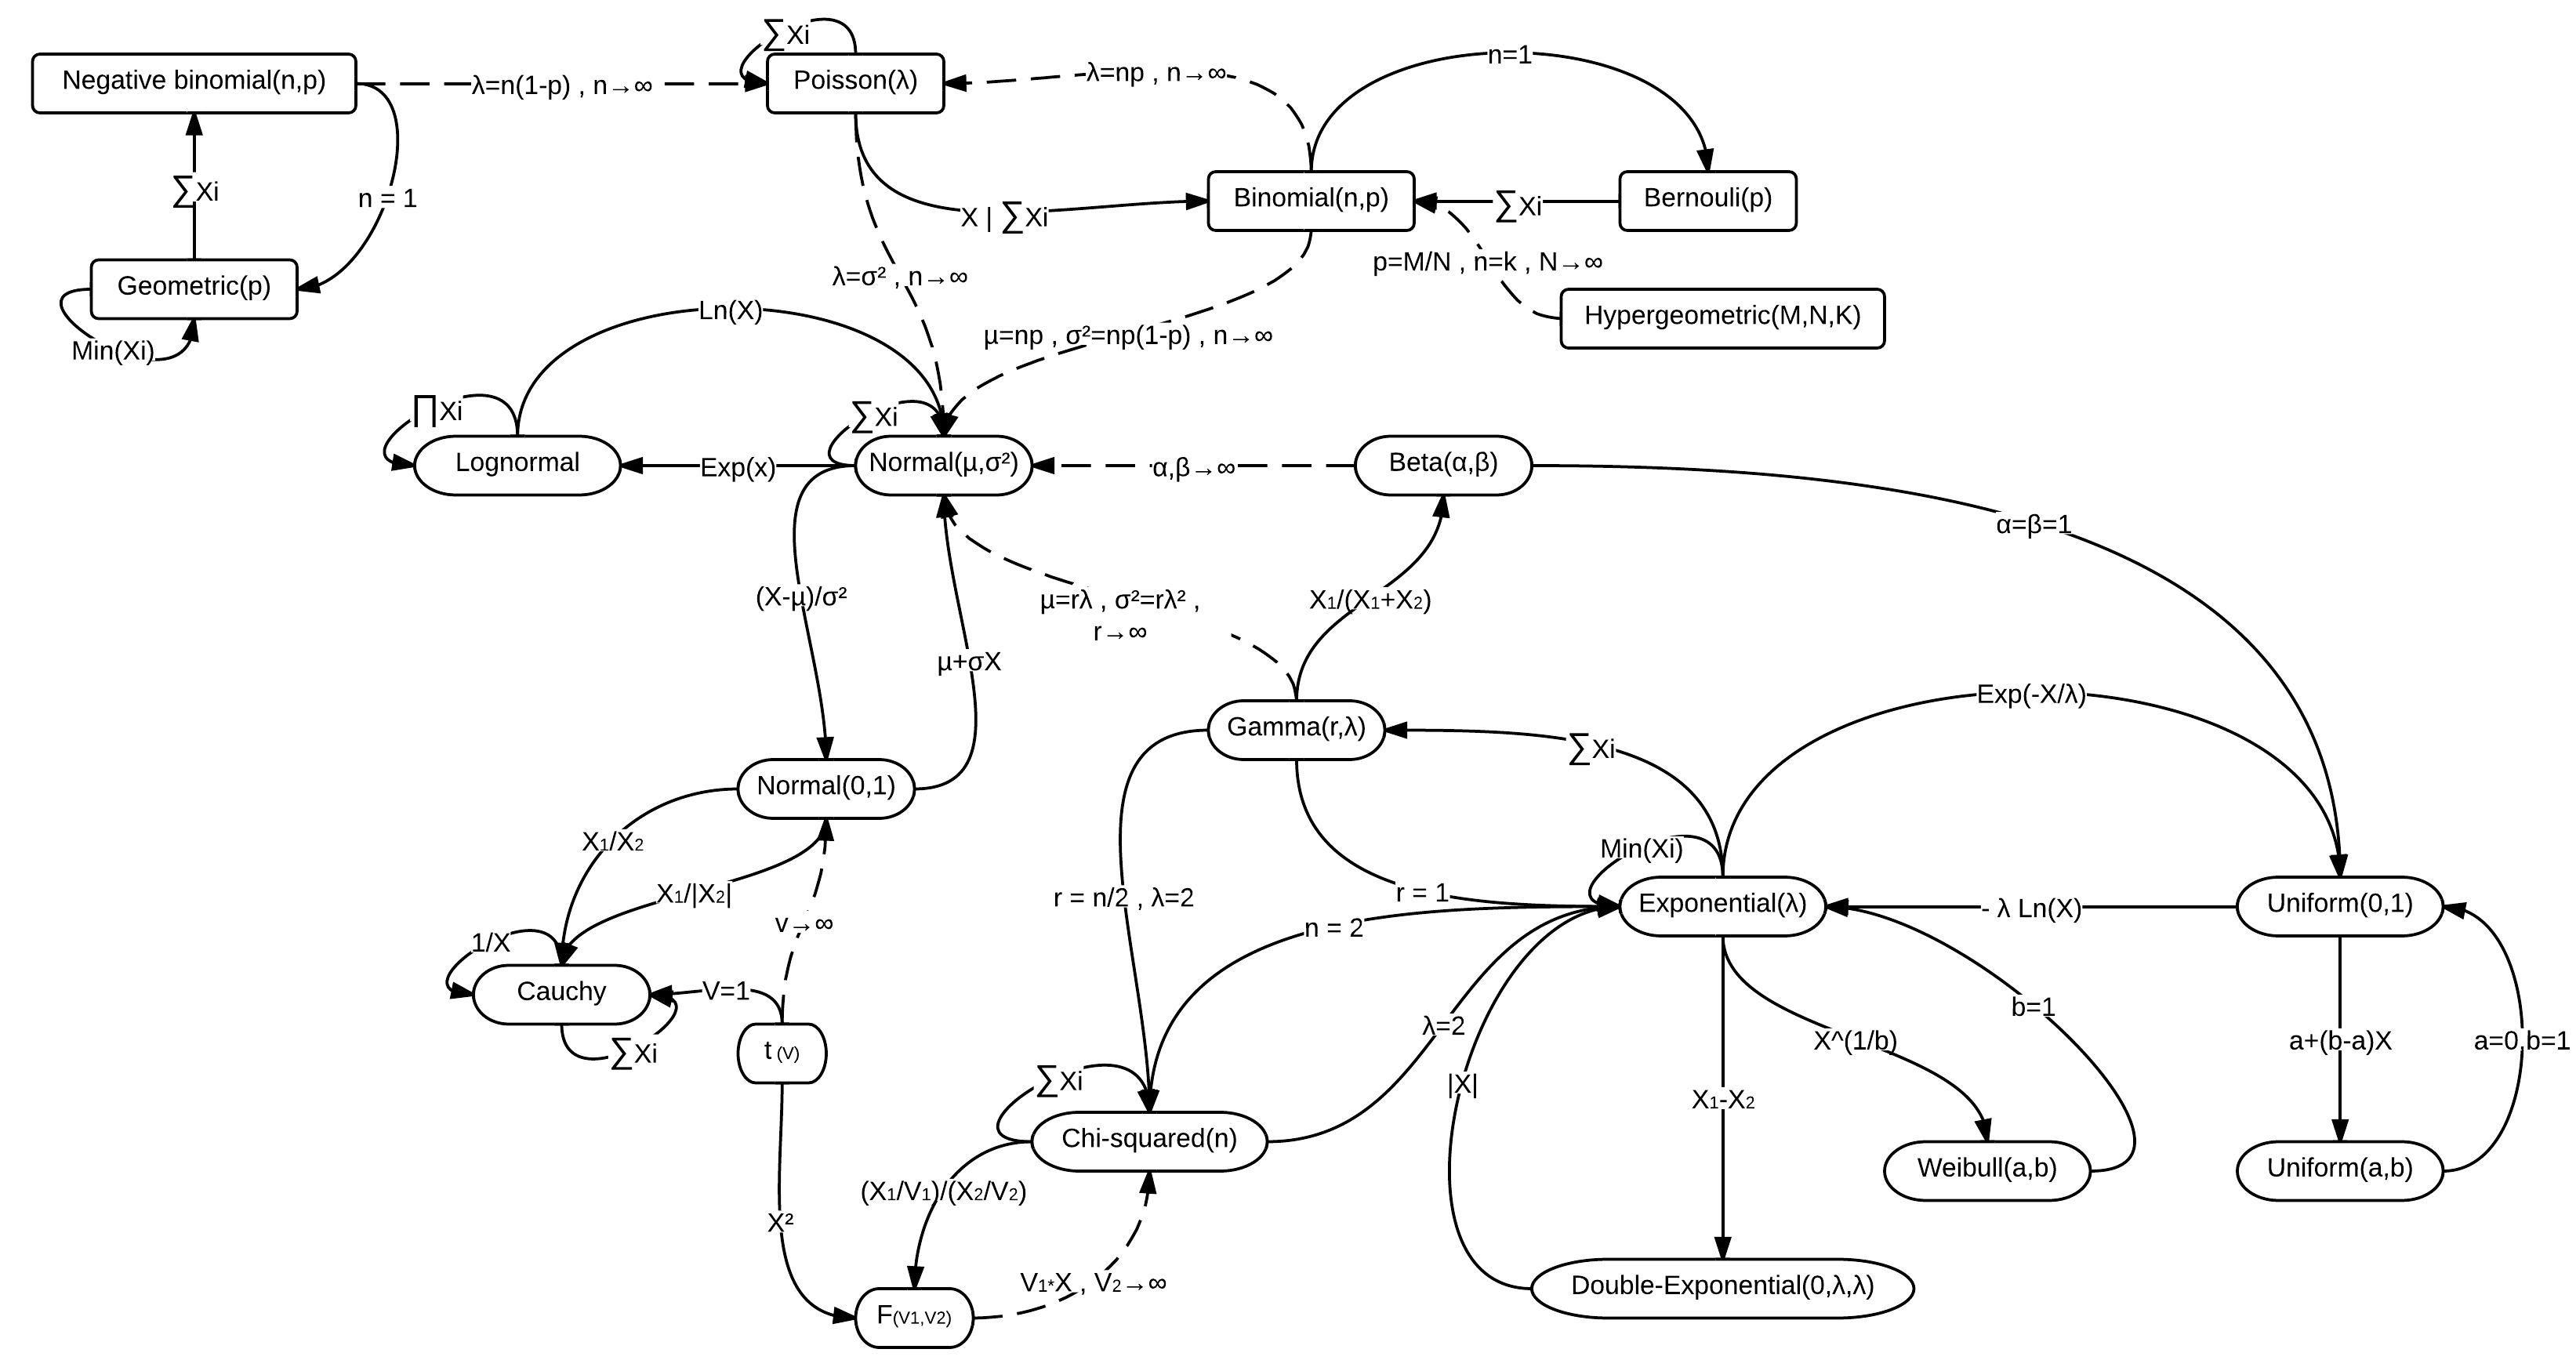
\includegraphics[width=0.7\textwidth]{../clipart/distribution_relations.jpeg}
    \end{figure}
  \end{frame}
\end{document}